\documentclass[addpoints,12pt]{exam}
\usepackage{amsmath, amssymb}
\usepackage{todonotes}
\linespread{1.1}
\usepackage{graphicx}
\usepackage{multirow}
\usepackage{moreverb}
\boxedpoints
\pointsinmargin
\usepackage[T5,T1]{fontenc}


%\printanswers
\noprintanswers

\pagestyle{headandfoot}
\runningheadrule
\runningheader{Econ 103}
              {Final Examination, Page \thepage\ of \numpages}
              {May 1st, 2018}

\runningfooter{Name: \rule{5cm}{0.4pt}}{}{Student ID \#: \rule{5cm}{0.4pt}}


%%%%%%%%%%%%%%%%%%%%%%%%%%%%%%%%%%%%%%%%%%%%%%%%%%%%%%%%%%%%%%%
\begin{document}

\begin{center}
\large
\sc{Final Examination\\ \normalsize Econ 103, Statistics for Economists \\ \vspace{0.5em} May 1st, 2018}

\vspace{1em}

\normalsize
\fbox{\begin{minipage}{0.51\textwidth}
\textbf{\small You have 120 minutes to complete this exam.
Graphing calculators, notes, and textbooks are not permitted. }\end{minipage}}


\end{center}
%%%%%%%%%%%%%%%%%%%%%%%%%%%%%%%%%%%%%%%%%%%%%%%%%%%%%%%%%%%%%%%


\vspace{2em}
\begin{center}
  \fbox{\fbox{\parbox{5.5in}{\centering
        I pledge that, in taking and preparing for this exam, I have abided by the University of Pennsylvania's Code of Academic Integrity. I am aware that any violations of the code will result in a failing grade for this course.}}}
\end{center}
\vspace{0.2in}
\makebox[\textwidth]{Name:\enspace\hrulefill}

\vspace{0.2in}
\noindent \makebox[\textwidth]{Student ID \#:\enspace\hrulefill}

\vspace{0.3in}
\noindent\makebox[\textwidth]{Signature:\enspace\hrulefill}

%\rule{1cm}{0.4pt}
\vspace{2em}

\begin{center}
  \gradetable[h][questions]
\end{center}

\vspace{2em}

\paragraph{Instructions:} Answer all questions in the space provided, continuing on the back of the page if you run out of space. Show your work for full credit but be aware that writing down irrelevant information will not gain you points. Be sure to sign the academic integrity statement above and to write your name and student ID number on \emph{each page} in the space provided. Make sure that you have all pages of the exam before starting.

\paragraph{Warning:} If you continue writing after we call time, even if this is only to fill in your name, twenty-five points will be deducted from your final score. In addition, two points will be deducted for each page on which you do not write your name and student ID.

%%%%%%%%%%%%%%%%%%%%%%%%%%%%%%%%%%%%%%%%%%%%%%%%%%%%%%%%%%%%%%%
\newpage

\begin{questions}

  \question Someone in San Jose California, a city with 1 million residents, has stolen a car.
  The incident was captured on video, providing a detailed description of the thief.
  One out of every 10,000 people in San Jose fits this description.
  The police spot Amy walking down the street; she meets every detail of the description, so they arrest her.
  The only evidence against Amy is that she fits the description.
  The prosecutor argues as follows:
  \begin{quote}
    %It's true that the only evidence we have against Amy is that she matches the description of the thief provided by the video.
    It is \emph{highly} unlikely (far beyond a reasonable doubt) that an innocent person would fit this description.
    Hence, it is highly unlikely that Amy is innocent.
  \end{quote}
  %In this question you will use what you have learned about probability in Econ 103 to evaluate the prosecutor's argument.
  In parts (b)--(d) below, let $I$ denote the event that someone from San Jose is innocent of the theft, and $D$ be the event that she fits the description from the video.
\begin{parts}
  \part[5] How many of the residents of San Jose fit the description from the video?
  \begin{solution}[0.75in]
    There are 1 million people in San Jose.
    One out of every 10,000 fits the description.
    Thus, $1000000/10000 = 100$ people fit the description.
  \end{solution}
  \part[5] Calculate $P(I \cap D)$.
  \begin{solution}[0.75in]
    Of the 100 people in San Jose who fit the description, 99 are innocent and one is guilty.
    Hence, $P(I\cap D) = 99/1000000$.
  \end{solution}
  \part[5] Calculate $P(D|I)$.
  \begin{solution}[0.75in]
    There are 1 million people in San Jose, and only one of them is guilty.
    Hence $P(I) = 999999/1000000$.
    By the definition of conditional probability,
    \begin{align*}
      P(D|I) = \frac{P(I \cap D)}{P(I)} = \frac{99/1000000}{999999/1000000} = \frac{99}{999999} \approx 1/10000
    \end{align*}
  \end{solution}
  \part[5] Calculate $P(I|D)$.
  \begin{solution}[0.75in]
    From above, 100 out of people in San Jose fit the description.
    Thus, $P(D) = 100/1000000$.
    By the definition of conditional probability,
    \begin{align*}
      P(I|D) = \frac{P(I \cap D)}{P(D)} = \frac{99/1000000}{100/1000000} = 99/100
    \end{align*}
  \end{solution}
  \part[5] In light of your responses to parts (c) and (d), evaluate the prosecutor's argument.
  Should the jury vote to convict Amy?
  Explain briefly.
  \begin{solution}[2in]
    The jury should \emph{not} vote to convict Amy.
    The prosecutor is correct that, given someone is innocent, it is highly unlikely that she will fit the description: this probability is $P(D|I) \approx 1/10000$.
    The relevant probability, however, is the \emph{reverse} conditional probability, namely the probability that someone is innocent given that she fits the description.
    This is $P(I|D) = 99/100$ so it is \emph{highly likely} that Amy is innocent.
    The prosecutor's reasoning is fallacious.
    (FYI: this fallacy is commonly called the ``prosecutor's fallacy.'')
  \end{solution}
\end{parts}

  \question In this question you will determine the same probability two different ways: first by using the rules for calculating probabilities from class, and then by Monte Carlo simulation.
  %The probabilities we calculated for the Pepsi Challenge experiment correspond to what is called a ``Hypergeometric'' random variable.
  %The name is complicated, but the RV itself is fairly simple.
  %There is an urn containing $N$ balls.
  %$R$ of these balls are red.
  %You draw a subset of $n$ balls at random and \emph{without replacement} from the urn.
  %If we define $X$ to be the number of red balls that you obtain, then  $X\sim \mbox{Hypergeometric}(N,R,n)$.
  %To take a specific example, recall the Pepsi challenge experiment.
  %In this experiment there is a collection of $N=8$ cups of soda, $R=4$ of which contain Coke.
  %Our expert has to choose a subset of $n=4$ cups.
  %Accordingly, under the null hypothesis that she is guessing completely at random, the number of Cokes, $X$, among the four cups that she selects is a Hypergeometric$(N=8, R=4, n=4)$ random variable.
  \begin{parts}
    \part[10] There is an urn containing six balls, four of which are red.
    You make two random draws from the urn \emph{without replacement}.
    What is the probability that both of the balls you draw are red?
    %\part[2] What is the support set of a Hypergeometric$(N,R,n)$ random variable?
    %\begin{solution}[1.25in]
    %  $\left\{ 0, 1, \dots, n \right\}$
    %\end{solution}
    %\part[3] If order does not matter, how many different ways are there to choose a sample of $n$ balls from an urn containing $N$ balls?
    %\begin{solution}[1.25in]
    %  $\displaystyle{N \choose n}$
    %\end{solution}
    %\part[5] Suppose that $X\sim \mbox{Hypergeometric}(N=6,R=4,n=2)$.
    %Calculate $P(X = 2)$.
    \begin{solution}[3in]
      There are $\displaystyle{6 \choose 2} = \frac{6!}{4!2!} = 15$ ways to choose two balls from a collection of six balls, provided that order doesn't matter.
      This is the denominator in our probability calculation.
      For the numerator, we need to count how many of these 15 possible draws contain exactly two red balls.
      Since there are 4 red balls in the urn, there are $\displaystyle {4 \choose 2} = \frac{4!}{2!2!} = 6$ ways to choose 2 of them, so the probability is $6/15 = 0.4$.
    \end{solution}
    \part[15] Write R code to check your calculation from part (a) via Monte Carlo simulation using 10,000 simulation replications.
    %Your code should approximate the probability that you will get two red balls if you make two random draws without replacement from an urn containing six balls, four of which are red.
    For simplicity, I suggest that you create a vector called \texttt{urn} containing ones and zeros, where the ones represent the four red balls and the zeros represent the two other balls.
    You can then make random draws without replacement from \texttt{urn}.
    \begin{solution}[3.25in]
      \begin{verbatim}
urn = c(1, 1, 1, 1, 0, 0)
urn_sim = function() {
  draw = sample(urn, 2, replace = FALSE)
  sum(draw) == 2
}
sims = replicate(10000, urn_sim())
mean(sims) \end{verbatim}
    \end{solution}
  \end{parts}




  \question Let $X$ be a continuous RV with support set $[0,1]$ and pdf $f(x) = \alpha x^{\alpha-1}$ where $\alpha > 0$.
  \begin{parts}
    \part[10] Calculate the CDF of $X$.
    \begin{solution}[2.5in]
      \begin{align*}
        F(x_0) &= \int_{-\infty}^{x_0} f(x)\, dx = \alpha \int_{0}^{x_0} x^{\alpha-1}\, dx = \left. \frac{\alpha x^{\alpha}}{\alpha}\right|_{0}^{x_0} = x_0^\alpha
      \end{align*}
      So the CDF is $0$ for $x_0 < 0$, $x_0^\alpha$ for $x\in [0,1]$ and $1$ for $x_0 > 1$.
    \end{solution}
    \part[10] Calculate $E[X]$.
    \begin{solution}[2.5in]
      \begin{align*}
        E[X] &= \int_{-\infty}^{\infty} x f(x)\, dx = \alpha\int_0^1 x^\alpha\, dx = \left.\displaystyle\frac{\alpha x^{\alpha+1}}{\alpha + 1} \right|_{0}^1 = \frac{\alpha}{\alpha + 1}
      \end{align*}
    \end{solution}
    \part[10] Calculate $\mbox{Var}(X)$. You do not have to simplify your answer.
    \begin{solution}[2.75in]
      \begin{align*}
        E[X^2] &= \int_{-\infty}^{\infty} x^2 f(x)\, dx = \alpha\int_0^1 x^{\alpha+1}\, dx = \left. \frac{\alpha x^{\alpha + 2}}{\alpha + 2}\right|_0^1 = \frac{\alpha}{\alpha + 2}
      \end{align*}
      and by the shortcut rule,
      \begin{align*}
        \mbox{Var}(X) &= E[X^2] - \left(E[X]\right)^2  = \frac{\alpha}{\alpha + 2} - \left(\frac{\alpha}{\alpha + 1}\right)^2\\
        &= \frac{\alpha(\alpha + 1)^2 - \alpha^2 (\alpha + 2)}{(\alpha + 2)(\alpha + 1)^2} = \frac{\alpha}{(\alpha + 2) (\alpha + 1)^2}
      \end{align*}
    \end{solution}
  \end{parts}





  \question Let $X_1, \dots, X_n \sim \mbox{iid N}(\mu, \sigma^2)$ where $\sigma^2$ is known.
  In class we derived a $(1- \alpha)\times 100\%$ confidence interval for $\mu$ that takes the form $\mbox{Estimator} \pm \mbox{ME}$.
  This is called a \emph{two-sided} confidence interval, because it has two finite endpoints.
  It is also possible to construct \emph{one-sided} confidence intervals, although we did not consider these in Econ 103.
  An \emph{upper one-sided confidence interval} for a some parameter $\theta$ is defined as a range $[\mbox{LCL}, +\infty)$ constructed from the sample data such that $P(\mbox{LCL} \leq \theta) = 1 - \alpha$.
    In other words, the interval $[\mbox{LCL}, +\infty)$ covers $\theta$ with probability $1 - \alpha$.
      In this problem you will construct an upper one-sided confidence interval for $\mu$ based on $X_1, \dots, X_n$.
  \begin{parts}
    \part[5] What is the sampling distribution of $\sqrt{n}(\bar{X}_n - \mu)/\sigma$?
    Be sure to specify the values of any and all parameters of its distribution.
    \begin{solution}[0.75in]
      $N(0,1)$
    \end{solution}
    \part[5] Continuing from the preceding part, write down the line of R code we would use to find the value of $c$ such that $P\big(\sqrt{n}(\bar{X}_n - \mu)/\sigma \leq c\big) = 1 - \alpha$.
    \begin{solution}[1.5in]
      Let $Z = \sqrt{n}(\bar{X}_n - \mu) / \sigma$.
      We need to find $c$ so that $P(Z\leq c) = 1 - \alpha$.
      Since $Z \sim N(0,1)$,  $c = \texttt{qnorm}(1 - \alpha)$.
    \end{solution}
    \part[10]
    %By rearranging the expression $P\big(\sqrt{n}(\bar{X}_n - \mu)/\sigma \leq c\big) = 1 - \alpha$,
    Using the expression from (b), derive the formula for LCL such that $[\mbox{LCL}, +\infty)$ is an upper one-sided confidence interval for $\mu$ with confidence level $(1 - \alpha)$.
      \begin{solution}[3.25in]
        Re-arranging the expression from (b),
        \begin{align*}
          P\left( \sqrt{n}(\bar{X}_n - \mu)/\sigma \leq c \right) &= 1 - \alpha\\
          P\left( - \mu \leq c \sigma/\sqrt{n} - \bar{X}_n \right) &= 1 - \alpha\\
          P\left(\mu \geq \bar{X}_n - c \sigma/\sqrt{n}\right) &= 1 - \alpha\\
          P\left(\bar{X}_n - c \sigma/\sqrt{n} \leq \mu\right) &= 1 - \alpha
        \end{align*}
        Hence, $\mbox{LCL} = \bar{X}_n - c\sigma/\sqrt{n}$ where $c = \texttt{qnorm}(1 - \alpha)$ by part (b).
      \end{solution}
  \end{parts}



\question This question is taken from your homework.
It is based on a dataset containing the results of the tae kwon do event in the 2004 Athens Olympics.
%(In case this event is unfamiliar to you, my dictionary defines tae kwon do as ``a modern Korean martial art similar to karate.'')
The competition is a tournament consisting of a number of bouts.
In each bout, a pair of competitors fight each other, points are awarded, and a winner is declared by the judges.
In accordance with Olympic regulations, one of the competitors in each bout is \emph{randomly chosen} to wear blue body protectors.
The other wears red body protectors.
This question investigates whether wearing one color or the other gives an advantage in the competition.
The data are stored in a data table called \texttt{taekwondo}.
Each row corresponds to a \emph{single bout}:

\small
\fbox{
	\begin{tabular}{ll}
		%\texttt{class}& weight class of the bout\\
		\texttt{red.id} & competitor id number for the fighter who wore red\\
		\texttt{blue.id} & competitor id number for the fighter who wore blue\\
		\texttt{round}& round of the tournament (i.e.\ semifinals, finals, etc.)\\
		\texttt{winner} & color worn by the fighter who won the bout\\
		\texttt{method} & method of win (i.e.\ points, knockout, etc.)\\
		\texttt{red.points} & number of points awarded to the fighter who wore red\\
		\texttt{blue.points} & number of points awarded to the fighter who wore blue
	\end{tabular}}
  \normalsize

There are no missing values in the dataset.
Here are the first few rows:
\small
\begin{verbatim}
   red.id blue.id   round winner  method   red.points blue.points
1:   5816    5818 last 16   Blue  Points            9           5
2:   5817    5824 last 16   Blue  Points            3           5
3:   5819    5825 last 16    Red  Points           15          16
4:   5820    5822 last 16    Red  Points           14          15
5:   5821    5827 last 16    Red  Points           13          12
6:   5828    5823 last 16    Red  Knockout          7           3
\end{verbatim}
\normalsize

	\begin{parts}
		\part[4] We'll restrict attention to the ``last 16'' round of the competition to ensure that each row contains a \emph{unique} pair of fighters. Write R code to extract only those rows of \texttt{taekwondo} for which the value in the column \texttt{round} is ``last 16'' and store the result in a data table called \texttt{last16}.
			\begin{solution}[0.75in]
				\begin{verbatim}
				last16 = taekwondo[round == "last 16"]
				\end{verbatim}
			\end{solution}
		\part[6] To begin, we'll analyze the \emph{proportion} of bouts won by the blue fighter. Write R code to: (i) count the number of elements in the column \texttt{winner} of \texttt{last16} and store the result in a variable called \texttt{n}, and (ii) count the number of bouts won by the blue fighter and store the result in a variable called \texttt{n.blue}.
			\begin{solution}[1in]
				\begin{verbatim}
n = last16[, length(winner)]
n.blue = last16[, sum(winner == `Blue')]
				\end{verbatim}
			\end{solution}
		\part[10] There are 32 bouts in \texttt{last16} of which 19 were won by the blue fighter. Using this information, calculate an approximate 95\% confidence interval for the population proportion of bouts won by fighters wearing blue based on the approximation provided by the CLT.
    Do your results suggest that wearing one color versus the other conveys a competitive advantage? Explain briefly.
			\begin{solution}[2.25in]
				\begin{eqnarray*}
					\widehat{p} &=& 19/32 \approx 0.59\\
					\tilde{SE}(\widehat{p}) &=& \sqrt{\widehat{p}(1 - \widehat{p})/n} = \sqrt{\left(\frac{19}{32} \times \frac{13}{32}\right)/32}\approx 0.09
				\end{eqnarray*}
				Hence, the CI is approximately $0.59 \pm 2\times 0.09$ or roughly $(0.41, 0.77)$.
        We do not find convincing evidence that either color conveys an advantage.
        If we absolutely had to guess, we would say that blue might convey a slight advantage but our results are perfectly consistent with the reverse as well: the difference between the estimated proportion and 0.5 could easily be nothing more than sampling variability.
			\end{solution}
		\part[10] Now suppose that you wanted to test the null hypothesis that the population proportion of bouts won by fighters wearing blue equals 0.5 against the two-sided alternative.
    Approximately what is your p-value for this test? Explain your results.
			\begin{solution}[2.25in]
				The test statistic is:
				$$T = \frac{\widehat{p} - 0.5}{\sqrt{0.5^2/n}} = \frac{19/32 - 0.5}{\sqrt{0.25/32}} \approx 1.06$$
				If the test statistic were \emph{exactly} one, the p-value for a two-sided test would be \texttt{2 * (1 - pnorm(1))}$\approx 2 \times 0.16 = 0.32$. The test statistic here is slightly larger than one, so the p-value should be slightly smaller than 0.32. This is a very large p-value: we would \emph{fail} to reject the null at any of the standard significance levels (i.e.\ 10\%, 5\%, 1\%). We have not found convincing evidence that wearing either color conveys a competitive advantage.
			\end{solution}
      \part[6] For the remainder of the question, we will examine the relative difference in the number of \emph{points} scored by the blue and red fighters in each bout. Write R code accomplish the following: (i) select only those rows of \texttt{last16} for which the value in the column \texttt{method} is \texttt{Points} and store the result in a data table called \texttt{last16.points}, (ii) create a vector called \texttt{D} whose entries contain the \emph{difference} in the number of points scored by blue versus red (Blue - Red) in each bout with \texttt{method} equal to \texttt{Points}.
			\begin{solution}[1in]
				\begin{verbatim}
last16.points = last16[method == `Points']
D = last16.points[, blue.points - red.points]
				\end{verbatim}
			\end{solution}
		\part[4] I calculated the mean of the column \texttt{red.points} in \texttt{last16.points} and got 10.1. Similarly, I calculated the mean of the column \texttt{blue.points} and got 11.7. If I were to run the command \texttt{mean(D)} at the R console what result would I get?
		\begin{solution}[0.75in]
			$11.7 - 10.1 = 1.6$
		\end{solution}
		\part[10] I entered the command \texttt{var(D)} at the R console and got 25. Next I entered \texttt{var(last16.points\$red.points)} and \texttt{var(last16.points\$blue.points)} and got 17 and 31, respectively. Calculate the sample correlation between the columns \texttt{red.points} and \texttt{blue.points} of the data table \texttt{last16.points}.
			\begin{solution}[2.5in]
			Rearranging the formula from class and substituting values from the question statement:
				\begin{eqnarray*}
			s_d^2 &=& s_x^2 + s_y^2	- 2s_x s_y r_{xy}\\
			2s_x s_y r_{xy} &=& s_x^2 + s_y^2 - s_d^2\\
			r_{xy} &=& \frac{s_x^2 + s_y^2 - s_d^2}{2s_x s_y}\\ \\
				&=& \frac{17 + 31 - 25}{2\sqrt{17 \times 31}} = \frac{23}{2 \times \sqrt{527}} \approx 0.5
				\end{eqnarray*}
			\end{solution}
		\part[10] To test the null hypothesis that red and blue fighters are awarded, on average, the same number of points against the two-sided alternative, should we use a test for independent samples or matched pairs data? Explain briefly and then carry out the appropriate test at the 5\% level based on the CLT. To answer, you will need the fact that there are 29 rows in the data table \texttt{last16.points}. Be sure to report: (i) the test statistic, (ii) the decision rule, and (iii) the result of the test.
			\begin{solution}[2.5in]
				This is matched pairs data: the score earned by the red fighter in a given bout cannot possibly be independent of the score earned by the blue fighter \emph{in the same bout}. The test statistic is
					$$T = \frac{\bar{D}}{s_d/\sqrt{n}} = 1.6 / (5/\sqrt{29}) \approx 1.7$$
				For a 5\% test, the decision rule is: Reject $H_0$ if $|T|>2$. In this case we fail to reject the null hypothesis.
			\end{solution}
	\end{parts}



  \question This question is based on a data table called \texttt{face} containing data from a paper investigating whether ``inferences of competence based solely on facial appearance predicted the outcomes of U.S.\ congressional outcomes.''
  Here are the first few rows of the dataset:
\begin{verbatim}
   year state     Dcomp    Dshare blueState
1: 2002    AK 0.3335918 0.1166021         0
2: 2004    AK 0.4193548 0.4777151         0
3: 2002    AL 0.5510950 0.4048368         0
4: 2004    AL 0.3223141 0.3236140         0
5: 2002    AR 0.2738834 0.5386246         0
6: 2004    AR 0.7360000 0.5582051         0
\end{verbatim}
Each row corresponds to a particular U.S.\ congressional election: \texttt{year} gives the year of the election, \texttt{state} gives the state, and \texttt{Dshare} gives the Democratic vote share.
For example, the value of $0.1166021$ for \texttt{Dshare} in the first row indicates that the Democratic candidate in the 2002 congressional race in Alaska got just under 12\% of the vote.
The column \texttt{blueState} is a dummy variable taking the value 1 if the corresponding state is a ``blue state,'' defined as a state in which most voters have favored the Democratic presidential candidate in past elections.
We see from the first six rows of this dataset that Alaska (AK), Alabama (AL), and Arkansas (AR), are \emph{red states}.
The column \texttt{Dcomp} is a measure of the ``facial competence'' of the Democratic congressional candidate, constructed as follows.
For each congressional race, a group of students were shown \emph{unlabeled} photographs of the Democratic and Republican candidates side-by-side:
\begin{center}
  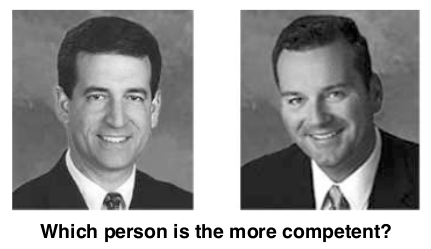
\includegraphics[scale = 0.4]{facial-competence.png}
\end{center}
After viewing the photographs for one second, the students were asked which person appeared more competent, based on the photographs.
The variable \texttt{Dcomp} records the \emph{fraction} of students who thought that the Democratic candidate appeared more competent.
For example, the value of 0.3335918 for \texttt{Dcomp} in the first row of \texttt{face} indicates that just over a third of the students thought that the Democratic candidate from the 2002 Alaska congressional race appeared more competent than his Republican rival.
Any student who recognized either photograph was excluded from the calculation, so that \texttt{Dcomp} is constructed purely ``based on judgements derived from facial appearance in the absence of prior knowledge about the person.''
To be clear: the students did not know that the people in the photos were congressional candidates, or which was a Democrat.

\newpage

To answer the following parts you will need to refer to the regression results on the final page of this exam.
You may want to tear out that page for ease of reference.
\begin{parts}
  \part[5] What is the sample correlation between \texttt{Dcomp} and \texttt{Dshare}?
  \begin{solution}[1in]
    The R-squared from Regression \#1 equals 0.19 and gives the \emph{square} of this correlation.
    The correlation itself equals $\sqrt{0.19} \approx 0.44$.
  \end{solution}
  \part[5] Construct an approximate 95\% confidence for the slope in a linear regression in which \texttt{Dcomp} \emph{alone} is used to predict \texttt{Dshare}.
  Briefly interpret your results.
  \begin{solution}[2in]
    From the results of Regression \#1, our estimate of the slope is 0.33 with a standard error of 0.06.
    Thus, the approximate 95\% confidence interval is $0.33 \pm 0.12$ or $(0.21, 0.33)$.
    There is a \emph{strong} positive relationship between \texttt{Dcomp} and \texttt{Dshare}.
  \end{solution}
  \part[5] Continuing from the previous part, how accurately does \texttt{Dcomp} predict \texttt{Dshare}?
  \begin{solution}[1in]
    The residual standard deviation from Regression \#1 is 0.13, indicating that \texttt{Dcomp} predicts \texttt{Dshare} to an accuracy of about 13 percentage points.
  \end{solution}
  \part[5] Suppose you wanted to test the null hypothesis that Democratic congressional candidates do equally well, in terms of vote share, in blue and red states against the two-sided alternative.
  What is the value of your test statistic?
  Approximately that is the p-value of the test?
  Briefly interpret your results.
  \begin{solution}[2.25in]
    Using the results of Regression \#2, the test statistic is $0.12 / 0.03 = 4$ yielding a p-value of less than 0.01.
    There is very strong evidence that Democratic congressional candidates do better (i.e.\ have a higher vote share) in blue states compared to red states.
  \end{solution}
  \part[5] Is there evidence that the relationship between \texttt{Dcomp} and \texttt{Dshare} differs in red and blue states?
  Justify your answer.
  \begin{solution}[2in]
    For full points, an answer should point out that we need to look at estimate of the interaction term \texttt{blueState:Dcomp} in Regression \#4.
    It should explain the meaning of the point estimate of -0.18, namely that the estimated slope is \emph{smaller} in blue states, but also point out that the standard error is large.
    This difference could easily be due to sampling variability, a point that could be made either with a confidence interval or hypothesis test.
  \end{solution}
  \part[15] Based on the full set of regression results, do you agree with the claim that ``inferences of competence from faces predict election outcomes?''
  Justify your answer using the tools you have learned in Econ 103.
  Clear, concise answers will be treated more favorably than long-winded ones.
  \begin{solution}
    For full points, students should recognize that they need to examine the results of Regressions \#1, \#3, and \#4.
    They should explain what each of these regressions tells us and point out that even after we control for \texttt{blueState}, either with or without an interaction, there is a strong positive relationship between \texttt{Dcomp} and \texttt{Dshare}.
    Facial competence clearly does predict results in US congressional elections.
    A complete answer should rely on statistical inferences to support this claim: either confidence intervals, hypothesis tests, or both.
  \end{solution}

\end{parts}





\newpage
\footnotesize
\paragraph{\footnotesize Regression \#1}
\begin{boxedverbatim}
lm(formula = Dshare ~ Dcomp, data = face)
            coef.est coef.se
(Intercept) 0.34     0.03
Dcomp       0.33     0.06
---
n = 118, k = 2
residual sd = 0.13, R-Squared = 0.19
\end{boxedverbatim}
\vspace{-1em}

\paragraph{\footnotesize Regression \#2}
\begin{boxedverbatim}
lm(formula = Dshare ~ blueState, data = face)
            coef.est coef.se
(Intercept) 0.46     0.02
blueState   0.12     0.03
---
n = 118, k = 2
residual sd = 0.14, R-Squared = 0.15
\end{boxedverbatim}
\vspace{-1em}

\paragraph{\footnotesize Regression \#3}
\begin{boxedverbatim}
lm(formula = Dshare ~ blueState + Dcomp, data = face)
            coef.est coef.se
(Intercept) 0.33     0.03
blueState   0.09     0.02
Dcomp       0.28     0.06
---
n = 118, k = 3
residual sd = 0.13, R-Squared = 0.27
\end{boxedverbatim}
\vspace{-1em}

\paragraph{\footnotesize Regression \#4}
\begin{boxedverbatim}
lm(formula = Dshare ~ blueState + Dcomp + blueState:Dcomp, data = face)
                coef.est coef.se
(Intercept)      0.30     0.04
blueState        0.18     0.07
Dcomp            0.35     0.08
blueState:Dcomp -0.18     0.13
---
n = 118, k = 4
residual sd = 0.13, R-Squared = 0.29
\end{boxedverbatim}


\end{questions}
\end{document}
